\documentclass[aspectratio=169]{beamer}
\usetheme{Boadilla}
%\usetheme{Warsaw}
%\setbeamercovered{transparent}
\beamertemplatetransparentcoveredhigh
\usepackage[portuges]{babel}
\usepackage[utf8]{inputenc}
\usepackage{lmodern}
\usepackage[T1]{fontenc}
\usepackage[portuguese, linesnumbered, vlined, titlenumbered, ruled]{algorithm2e}
\SetKwRepeat{Registro}{registro \{}{\}}%
\usepackage{hyperref} 

\usepackage{xcolor}
\definecolor{codegreen}{rgb}{0,0.6,0}
\definecolor{codegray}{rgb}{0.5,0.5,0.5}
\definecolor{codepurple}{rgb}{0.58,0,0.82}
\definecolor{backcolour}{rgb}{0.95,0.95,0.92}

\usepackage{listings}
\lstdefinestyle{CStyle}{
    language=C++,
    backgroundcolor=\color{backcolour},   
    commentstyle=\color{codegreen},
    keywordstyle=\color{magenta},
    numberstyle=\tiny\color{codegray},
    stringstyle=\color{codepurple},
    basicstyle=\ttfamily\footnotesize,
    breakatwhitespace=false,         
    breaklines=true,                 
    keepspaces=true,                 
    numbers=left,       
    numbersep=5pt,                  
    showspaces=false,                
    showstringspaces=false,
    showtabs=false,                  
    tabsize=2,
}

\newcommand{\eng}[1]{\textsl{#1}}
\newcommand{\cod}[1]{\texttt{#1}}

\title[Aula Prática Pilha e Fila]{Pilha, Fila\\
   Algoritmos e Estrutura de Dados}
\subtitle{Pilha e Fila\\(Alocação Dinâmica)}
\author[Frederico Santos de Oliveira]{prof. Frederico Santos de Oliveira}
\institute[UFMT]{Universidade Federal de Mato Grosso\\ Instituto de Engenharia}
\date{}

\AtBeginSection[]
{
	\begin{frame}
	\frametitle{Roteiro da Aula}
	\tableofcontents[currentsection]
\end{frame}
}


\begin{document}

\begin{frame}[plain]
  \titlepage
\end{frame}

%\section*{Roteiro}

%\begin{frame}
%  \frametitle{Agenda}
%  \tableofcontents
%\end{frame}

%%%%%%%%%%%%%%%%%%%%%%%%%%%%%%%%%%%%%%%%%%%%%%%%%%%%%%%%%%%%%%%%%%%%%%%%%%%%%%%%%%%%%%%%
\section{Introdução}
%%%%%%%%%%%%%%%%%%%%%%%%%%%%%%%%%%%%%%%%%%%%%%%%%%%%%%%%%%%%%%%%%%%%%%%%%%%%%%%%%%%%%%%%

\begin{frame}{Introdução}{Estrutura Nodo}
\begin{itemize}
 \item A  entidade elementar de uma estrutura de dados é o nodo (nó). 
 \item Um nodo é diferenciado pelo seu endereço relativo dentro da estrutura  e pode ser constituído de um ou vários campos. 
 \item Cada campo de um nodo armazena uma informação, um dado, que pode ser do tipo numérico, alfanumérico, lógicos, imagens, sons, enfim, qualquer informação que possa ser manipulada. 
 \item Todos os nodos de uma mesma estrutura devem ter a mesma configuração. 
\end{itemize}
\end{frame}

%%%%%%%%%%%%%%%%%%%%%%%%%%%%%%%%%%%%%%%%%%%%%%%%%%%%%%%%%%%%%%%%%%%%%%%%%%%%%%%%%%%%%%%%

\begin{frame}{Introdução}{Estrutura Nodo}
Cada nodo armazena:
\begin{itemize}
 \item Um elemento.
  \begin{itemize}
  \item pode ser um inteiro, uma string, um vetor, um registro, não importa. 
  \item Aqui é denominado apenas {\bf item}.
  \end{itemize}  
 \item Uma ligação para o próximo nodo. 
 \begin{itemize}
 \item Em termos de implementação, trata-se de um ponteiro do tipo nodo, o qual denominaremos {\bf prox}.
 \end{itemize}
 \end{itemize}
\begin{figure}[!h]
  \centering
   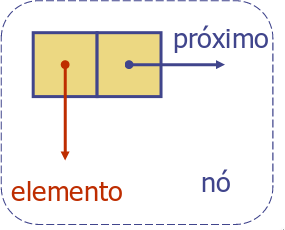
\includegraphics[width=100pt]{imagens/nodo.png}
  \label{fig_introducao}
\end{figure}
\end{frame}

%%%%%%%%%%%%%%%%%%%%%%%%%%%%%%%%%%%%%%%%%%%%%%%%%%%%%%%%%%%%%%%%%%%%%%%%%%%%%%%%%%%%%%%%

\begin{frame}[fragile]{Introdução}{Estrutura Nodo}
Primeiramente, vamos implementar o tipo de dados \verb|nodo|. Vamos analisar o pseudo-código apresentado nas aulas anteriores.
\end{frame}

%%%%%%%%%%%%%%%%%%%%%%%%%%%%%%%%%%%%%%%%%%%%%%%%%%%%%%%%%%%%%%%%%%%%%%%%%%%%%%%%%%%%%%%%

\begin{frame}[fragile]{Introdução}{Estrutura Nodo}
\begin{algorithm}[H]
\caption{Nodo} 
\label{Nodo}
\Inicio{
 \Registro{Nodo}{
    Inteiro: item; \\
    Ponteiro Nodo: prox; 
  }
}
\end{algorithm} 
\end{frame}

%%%%%%%%%%%%%%%%%%%%%%%%%%%%%%%%%%%%%%%%%%%%%%%%%%%%%%%%%%%%%%%%%%%%%%%%%%%%%%%%%%%%%%%%%%%%%%%%%%%%%

\begin{frame}[fragile]{Introdução}{Estrutura Nodo}
Na linguagem C, a implementação fica conforme o código a seguir:
\begin{lstlisting}[style=CStyle]
typedef struct nodo_t {
    int item;
    struct nodo_t *prox; 
} nodo;
\end{lstlisting}  
Vamos chamar o arquivo que contém esse código de \verb|nodo.h|.
\end{frame}

%%%%%%%%%%%%%%%%%%%%%%%%%%%%%%%%%%%%%%%%%%%%%%%%%%%%%%%%%%%%%%%%%%%%%%%%%%%%%%%%%%%%%%%%
\section{Exercício 1}
%%%%%%%%%%%%%%%%%%%%%%%%%%%%%%%%%%%%%%%%%%%%%%%%%%%%%%%%%%%%%%%%%%%%%%%%%%%%%%%%%%%%%%%%

\begin{frame}[fragile]{Exercício 2}{Estrutura Pilha}
Neste exercício, vamos implementar a estrutura de dados {\bf Pilha}:
\begin{itemize}
 \item Nessa estrutura existem dois ponteiros:
 \begin{itemize}
    \item um aponta para o {\bf topo} da Pilha.
    \item o outro que aponta para o {\bf fundo} da Pilha.
 \end{itemize}
 \item No topo da Pilha existe um nodo vazio (denominado nodo {\bf cabeça}).
 \item O ponteiro topo sempre aponta para o nodo cabeça.
 \item Quando a Pilha está vazia, fundo e topo apontam para o nodo cabeça.
\end{itemize}
\end{frame}

%%%%%%%%%%%%%%%%%%%%%%%%%%%%%%%%%%%%%%%%%%%%%%%%%%%%%%%%%%%%%%%%%%%%%%%%%%%%%%%%%%%%%%%%%%%%%%%%%%%%%

\begin{frame}[fragile]{Exercício 2}{Pilha}
Considere o pseudo-código a seguir:
\begin{algorithm}[H]
\caption{Pilha} 
\label{Pilha}
\Inicio{
 \Registro{Pilha}{
    Ponteiro Nodo: topo, fundo; 
  }
}
\end{algorithm} 
\end{frame}

%%%%%%%%%%%%%%%%%%%%%%%%%%%%%%%%%%%%%%%%%%%%%%%%%%%%%%%%%%%%%%%%%%%%%%%%%%%%%%%%%%%%%%%%%%%%%%%%%%%%%

\begin{frame}[fragile]{Exercício 2}{Pilha}
Na linguagem C, a implementação fica conforme o código a seguir:
\begin{lstlisting}[style=CStyle]
#include "nodo.h"
typedef struct {
    nodo *topo, *fundo;
} pilha;
\end{lstlisting}  
Vamos chamar o arquivo que contém esse código de \verb|pilha.h|.
\end{frame}

%%%%%%%%%%%%%%%%%%%%%%%%%%%%%%%%%%%%%%%%%%%%%%%%%%%%%%%%%%%%%%%%%%%%%%%%%%%%%%%%%%%%%%%%%%%%%%%%%%%%%

\begin{frame}[fragile]{Exercício 2}{Pilha}
A seguir, vamos implementar cada uma das seguintes funções:
\begin{enumerate}
 \item CriaPilhaVazia($S$) 
 \item PilhaVazia($S$)
 \item Empilha($S$,$x$)
 \item Desempilha($S$) 
 \item ApagaPilha($S$)
\end{enumerate}
\end{frame}

%%%%%%%%%%%%%%%%%%%%%%%%%%%%%%%%%%%%%%%%%%%%%%%%%%%%%%%%%%%%%%%%%%%%%%%%%%%%%%%%%%%%%%%%%%%%%%%%%%%%%

\begin{frame}[fragile]{Exercício 2}{Pilha}
Vamos adicionar o protótipo de cada uma das funções no arquivo \verb|pilha.h|.
\begin{lstlisting}[style=CStyle]
void criaPilhaVazia(pilha *s);
int pilhaVazia(pilha *s);
void empilha(pilha *s, int x);
int desempilha(pilha *s);
void apagaPilha(pilha *s);
\end{lstlisting}  
Agora, vamos implementar cada uma dessas funções. 
\end{frame}

%%%%%%%%%%%%%%%%%%%%%%%%%%%%%%%%%%%%%%%%%%%%%%%%%%%%%%%%%%%%%%%%%%%%%%%%%%%%%%%%%%%%%%%%%%%%%%%%%%%%%

\begin{frame}[fragile]{Exercício 2}{Pilha}
\begin{itemize}
\item Primeiramente, vamos criar um arquivo chamado \verb|pilha.c| que deve conter a implementação dessas funções.
\item Para evitar que o compilador não encontre determinada função, vamos incluir o protótipo das funções, inserindo a linha de código a seguir no início do arquivo \verb|pilha.c|:
\begin{lstlisting}[style=CStyle]
#include "pilha.h"
\end{lstlisting}  
\item A seguir, é apresentado a implementação das funções, que devem ser incluídas no arquivo \verb|pilha.c|.
\end{itemize}
\end{frame}

%%%%%%%%%%%%%%%%%%%%%%%%%%%%%%%%%%%%%%%%%%%%%%%%%%%%%%%%%%%%%%%%%%%%%%%%%%%%%%%%%%%%%%%%%%%%%%%%%%%%%

\begin{frame}[fragile]{Exercício 2}{Pilha}
% \scalebox{0.5}{
\begin{algorithm}[H]
\caption{CriaPilhaVazia} 
\label{CriaPilhaVazia}
\Entrada{Pilha S.}
\Inicio{
  S.topo $\leftarrow$ ALOCA\_NODO()\\
  S.fundo $\leftarrow$ S.topo\\
  S.topo.prox $\leftarrow$  NULL \\
%   $S.tamanho \leftarrow 0$ 
}
\end{algorithm}
\end{frame}

%%%%%%%%%%%%%%%%%%%%%%%%%%%%%%%%%%%%%%%%%%%%%%%%%%%%%%%%%%%%%%%%%%%%%%%%%%%%%%%%%%%%%%%%%%%%%%%%%%%%%

\begin{frame}[fragile]{Exercício 2}{Pilha}
Na linguagem C, a implementação fica conforme o código a seguir:
\begin{lstlisting}[style=CStyle]
void criaPilhaVazia(pilha *s) {
    s->topo = malloc(sizeof(nodo));
    s->fundo = s->topo;
    s->topo->prox = NULL;
}
\end{lstlisting}  
\end{frame}

%%%%%%%%%%%%%%%%%%%%%%%%%%%%%%%%%%%%%%%%%%%%%%%%%%%%%%%%%%%%%%%%%%%%%%%%%%%%%%%%%%%%%%%%%%%%%%%%%%%%%

\begin{frame}[fragile]{Exercício 2}{Pilha}
% \scalebox{0.5}{
\begin{algorithm}[H]
\caption{PilhaVazia} 
\label{PilhaVazia}
\Entrada{Pilha S.}
\Saida{Booleano (V ou F) indicando se S está vazia.}
\Inicio{
  \Se { (S.topo = S.fundo) } {
    \Retorna Verdadeiro \\
    }
  \Senao {
    \Retorna Falso
  } 
}
\end{algorithm}
% }  
\end{frame}

%%%%%%%%%%%%%%%%%%%%%%%%%%%%%%%%%%%%%%%%%%%%%%%%%%%%%%%%%%%%%%%%%%%%%%%%%%%%%%%%%%%%%%%%%%%%%%%%%%%%%

\begin{frame}[fragile]{Exercício 2}{Pilha}
Na linguagem C, a implementação fica conforme o código a seguir:
\begin{lstlisting}[style=CStyle]
int pilhaVazia(pilha *s) {
    return s->topo == s->fundo;
}
\end{lstlisting}  
\end{frame}

%%%%%%%%%%%%%%%%%%%%%%%%%%%%%%%%%%%%%%%%%%%%%%%%%%%%%%%%%%%%%%%%%%%%%%%%%%%%%%%%%%%%%%%%%%%%%%%%%%%%%

\begin{frame}[fragile]{Exercício 2}{Pilha}
% \scalebox{0.5}{
\begin{algorithm}[H]
\caption{Empilha} 
\label{Empilha}
\Entrada{Pilha S, item x.}
\Inicio{
  novo $\leftarrow$ ALOCA\_NODO() \\
  novo.prox $\leftarrow$ S.topo \\
  S.topo.item $\leftarrow$ x \\  
  S.topo $\leftarrow$ novo \\
%   $p.tamanho \leftarrow p.tamanho + 1$
}
\end{algorithm}
% }  
\end{frame}

%%%%%%%%%%%%%%%%%%%%%%%%%%%%%%%%%%%%%%%%%%%%%%%%%%%%%%%%%%%%%%%%%%%%%%%%%%%%%%%%%%%%%%%%%%%%%%%%%%%%%

\begin{frame}[fragile]{Exercício 2}{Pilha}
Na linguagem C, a implementação fica conforme o código a seguir:
\begin{lstlisting}[style=CStyle]
void empilha(pilha *s, int x) {
    nodo *novo = malloc(sizeof(nodo));
    novo->prox = s->topo;
    s->topo->item = x;
    s->topo = novo;
}
\end{lstlisting}  
\end{frame}

%%%%%%%%%%%%%%%%%%%%%%%%%%%%%%%%%%%%%%%%%%%%%%%%%%%%%%%%%%%%%%%%%%%%%%%%%%%%%%%%%%%%%%%%%%%%%%%%%%%%%

\begin{frame}[fragile]{Exercício 2}{Pilha}
% \scalebox{0.5}{
\begin{algorithm}[H]
\caption{Desempilha} 
\label{Desempilha}
\Entrada{Pilha S.}
\Saida{Item desempilhado.}
\Inicio{
  \Se {(PilhaVazia(S))}  
  { 
    Imprima "Erro {\it underflow}: pilha vazia." \\ 
  }
  \Senao {
    aux $\leftarrow$ S.topo \\
    S.topo $\leftarrow$ aux.prox \\
    item $\leftarrow$ aux.prox.item \\
    DESALOCA\_NODO(aux)\\  
    \Retorna item
  }
%   $S.tamanho \leftarrow S.tamanho - 1$ 
}
\end{algorithm}
% }  
\end{frame}

%%%%%%%%%%%%%%%%%%%%%%%%%%%%%%%%%%%%%%%%%%%%%%%%%%%%%%%%%%%%%%%%%%%%%%%%%%%%%%%%%%%%%%%%%%%%%%%%%%%%%

\begin{frame}[fragile]{Exercício 2}{Pilha}
Na linguagem C, a implementação fica conforme o código a seguir:
\begin{lstlisting}[style=CStyle]
int desempilha(pilha *s) {
    int item = -1;
    if (pilhaVazia(s)) 
        printf("Underflow: pilha vazia.\n");
    else {
        nodo *aux = s->topo;
        s->topo = aux->prox;
        item = aux->prox->item;
        free(aux);
    }
    return item;    
}
\end{lstlisting}  
\end{frame}

%%%%%%%%%%%%%%%%%%%%%%%%%%%%%%%%%%%%%%%%%%%%%%%%%%%%%%%%%%%%%%%%%%%%%%%%%%%%%%%%%%%%%%%%%%%%%%%%%%%%%

\begin{frame}[fragile]{Exercício 2}{Pilha}
\begin{itemize}
\item Ainda falta uma função: aquela que apaga todos os nodos de uma pilha.
\item Vamos implementá-la a seguir.
\end{itemize}
\end{frame}

%%%%%%%%%%%%%%%%%%%%%%%%%%%%%%%%%%%%%%%%%%%%%%%%%%%%%%%%%%%%%%%%%%%%%%%%%%%%%%%%%%%%%%%%%%%%%%%%%%%%%

\begin{frame}[fragile]{Exercício 2}{Pilha}
% \scalebox{0.5}{
\begin{algorithm}[H]
\caption{ApagaPilha} 
\label{ApagaPilha}
\Entrada{Pilha S.}
\Inicio{
  \Enqto {(NOT(PilhaVazia(S)))} {
    \CommentSty{// Ignora o elemento desempilhado.}\\
    Desempilha(S)\\
  }
  \CommentSty{// Apaga o nodo cabeça.}\\
  DESALOCA\_NODO(S.topo)\\
  S.topo $\leftarrow$ NULL \\
  S.fundo $\leftarrow$ NULL \\
%   $S.tamanho \leftarrow 0$ 
}
\end{algorithm}
% }  
\end{frame}

%%%%%%%%%%%%%%%%%%%%%%%%%%%%%%%%%%%%%%%%%%%%%%%%%%%%%%%%%%%%%%%%%%%%%%%%%%%%%%%%%%%%%%%%%%%%%%%%%%%%%

\begin{frame}[fragile]{Exercício 2}{Pilha}
Na linguagem C, a implementação fica conforme o código a seguir:
\begin{lstlisting}[style=CStyle]
void apagaPilha(pilha *s) {
    while (!pilhaVazia(s))
        desempilha(s); 
    free(s->topo);
    s->topo = NULL;
    s->fundo = NULL;
}  
\end{lstlisting}  
\end{frame}

%%%%%%%%%%%%%%%%%%%%%%%%%%%%%%%%%%%%%%%%%%%%%%%%%%%%%%%%%%%%%%%%%%%%%%%%%%%%%%%%%%%%%%%%%%%%%%%%%%%%%

\begin{frame}[fragile]{Exercício 2}{Pilha}
Após implementar essas funções, faça o teste, empilhando e desempilhando alguns valores.
\end{frame}

%%%%%%%%%%%%%%%%%%%%%%%%%%%%%%%%%%%%%%%%%%%%%%%%%%%%%%%%%%%%%%%%%%%%%%%%%%%%%%%%%%%%%%%%%%%%%%%%%%%%%

\begin{frame}[fragile]{Exercício 2}{Pilha}
Em um arquivo chamado \verb|executa_pilha.c|, insira  o código a seguir:
\begin{lstlisting}[style=CStyle]
#include "pilha.h"
int main() {
    int i;
    pilha *s = malloc(sizeof(pilha));
    criaPilhaVazia(s);
    for(i=0;i<10;i++) {
        empilha(s,i);
        printf("Empilhou %d\n",i);
    }
    while(!pilhaVazia(s)) {
        i = desempilha(s);
        printf("Desempilhou %d\n",i);    
    }
    apagaPilha(s);
    free(s);
}
\end{lstlisting}  
\end{frame}


%%%%%%%%%%%%%%%%%%%%%%%%%%%%%%%%%%%%%%%%%%%%%%%%%%%%%%%%%%%%%%%%%%%%%%%%%%%%%%%%%%%%%%%%%%%%%%%%%%%%%
\section{Exercício 2}
%%%%%%%%%%%%%%%%%%%%%%%%%%%%%%%%%%%%%%%%%%%%%%%%%%%%%%%%%%%%%%%%%%%%%%%%%%%%%%%%%%%%%%%%%%%%%%%%%%%%%

\begin{frame}[fragile]{Exercício 3}{Fila}
Neste exercício, vamos implementar a estrutura de dados {\bf Fila}:
\begin{itemize}
 \item Nessa estrutura existem dois ponteiros:
 \begin{itemize}
    \item um aponta para o {\bf início} da Fila.
    \item o outro que aponta para o {\bf fim} da Fila.
 \end{itemize}
 \item No início da Fila existe um nodo vazio (denominado nodo {\bf cabeça}).
 \item O ponteiro início sempre aponta para o nodo cabeça.
 \item Quando a Fila está vazia, início e fim apontam para o nodo cabeça.
\end{itemize}
\end{frame}

%%%%%%%%%%%%%%%%%%%%%%%%%%%%%%%%%%%%%%%%%%%%%%%%%%%%%%%%%%%%%%%%%%%%%%%%%%%%%%%%%%%%%%%%%%%%%%%%%%%%

\begin{frame}[fragile]{Exercício 3}{Fila}
Considere o pseudo-código a seguir:
\begin{algorithm}[H]
\caption{Fila} 
\label{Fila}
\Inicio{
 \Registro{Fila}{
    Ponteiro Nodo: início, fim; 
  }
}
\end{algorithm} 
\end{frame}

%%%%%%%%%%%%%%%%%%%%%%%%%%%%%%%%%%%%%%%%%%%%%%%%%%%%%%%%%%%%%%%%%%%%%%%%%%%%%%%%%%%%%%%%%%%%%%%%%%%%%

\begin{frame}[fragile]{Exercício 3}{Fila}
Na linguagem C, a implementação fica conforme o código a seguir:
\begin{lstlisting}[style=CStyle]
#include "nodo.h"
typedef struct {
    nodo *inicio, *fim;
} fila;
\end{lstlisting}  
Vamos chamar o arquivo que contém esse código de \verb|fila.h|.
\end{frame}


%%%%%%%%%%%%%%%%%%%%%%%%%%%%%%%%%%%%%%%%%%%%%%%%%%%%%%%%%%%%%%%%%%%%%%%%%%%%%%%%%%%%%%%%%%%%%%%%%%%%%

\begin{frame}{Exercício 3}{Fila}
Implemente uma fila utilizando alocação dinâmica. As operações básicas são:
\begin{enumerate}
 \item CriaFilaVazia($Q$) 
 \item FilaVazia($Q$)
 \item Enfileira($Q$,$x$)
 \item Desenfileira($Q$) 
 \item ApagaFila($Q$) 
\end{enumerate}
\end{frame}

%%%%%%%%%%%%%%%%%%%%%%%%%%%%%%%%%%%%%%%%%%%%%%%%%%%%%%%%%%%%%%%%%%%%%%%%%%%%%%%%%%%%%%%%%%%%%%%%%%%%%

\begin{frame}[fragile]{Exercício 3}{Fila}
Vamos adicionar o protótipo de cada uma das funções no arquivo \verb|fila.h|.
\begin{lstlisting}[style=CStyle]
void criaFilaVazia(fila *q);
int filaVazia(fila *q);
void enfileira(fila *q, int x);
int desenfileira(fila *q);
void apagaFila(fila *q);
\end{lstlisting}  
Agora, vamos implementar cada uma dessas funções. 
\end{frame}

%%%%%%%%%%%%%%%%%%%%%%%%%%%%%%%%%%%%%%%%%%%%%%%%%%%%%%%%%%%%%%%%%%%%%%%%%%%%%%%%%%%%%%%%%%%%%%%%%%%%%

\begin{frame}[fragile]{Exercício 3}{Fila}
\begin{itemize}
\item Primeiramente, de forma similar ao que fizemos com o TAD pilha, vamos criar um arquivo chamado \verb|fila.c| que deve conter a implementação dessas funções.
\item Para evitar que o compilador não encontre determinada função, vamos incluir o protótipo das funções, inserindo a linha de código a seguir no início do arquivo \verb|fila.c|:
\begin{lstlisting}[style=CStyle]
#include "fila.h"
\end{lstlisting}  
\item A seguir, é apresentado a implementação das funções, que devem ser incluídas no arquivo \verb|fila.c|.
\end{itemize}
\end{frame}

%%%%%%%%%%%%%%%%%%%%%%%%%%%%%%%%%%%%%%%%%%%%%%%%%%%%%%%%%%%%%%%%%%%%%%%%%%%%%%%%%%%%%%%%%%%%%%%%%%%%%

\begin{frame}[fragile]{Exercício 3}{Fila}
% \scalebox{0.5}{
\begin{algorithm}[H]
\caption{CriaFilaVazia} 
\label{CriaFilaVazia}
\Entrada{Fila Q.}
\Inicio{
  Q.inicio $\leftarrow$ ALOCA\_NODO() \\
  Q.fim $\leftarrow$ Q.inicio \\
  Q.inicio.prox $\leftarrow$ NULL
}
\end{algorithm}
% }  
\end{frame}

%%%%%%%%%%%%%%%%%%%%%%%%%%%%%%%%%%%%%%%%%%%%%%%%%%%%%%%%%%%%%%%%%%%%%%%%%%%%%%%%%%%%%%%%%%%%%%%%%%%%%

\begin{frame}[fragile]{Exercício 3}{Fila}
Na linguagem C, a implementação fica conforme o código a seguir:
\begin{lstlisting}[style=CStyle]
void criaFilaVazia(fila *q) {
    q->inicio = malloc(sizeof(nodo));
    q->fim = q->inicio;
    q->inicio->prox = NULL;
}
\end{lstlisting}  

\end{frame}

%%%%%%%%%%%%%%%%%%%%%%%%%%%%%%%%%%%%%%%%%%%%%%%%%%%%%%%%%%%%%%%%%%%%%%%%%%%%%%%%%%%%%%%%%%%%%%%%%%%%%

\begin{frame}[fragile]{Exercício 3}{Fila}
% \scalebox{0.5}{
\begin{algorithm}[H]
\caption{FilaVazia} 
\label{FilaVazia}
\Entrada{Fila Q.}
\Saida{Booleano (V ou F) indicando se Q está vazia.}
\Inicio{
  \Se {(Q.inicio = Q.fim)} {
  	\Retorna VERDADEIRO\\
  }
  \Senao{
    	\Retorna FALSO\\
  }
}
\end{algorithm}
% }  
\end{frame}

%%%%%%%%%%%%%%%%%%%%%%%%%%%%%%%%%%%%%%%%%%%%%%%%%%%%%%%%%%%%%%%%%%%%%%%%%%%%%%%%%%%%%%%%%%%%%%%%%%%%%

\begin{frame}[fragile]{Exercício 3}{Fila}
Na linguagem C, a implementação fica conforme o código a seguir:
\begin{lstlisting}[style=CStyle]
int filaVazia(fila *q) {
    return q->inicio == q->fim;
}
\end{lstlisting}  
\end{frame}

%%%%%%%%%%%%%%%%%%%%%%%%%%%%%%%%%%%%%%%%%%%%%%%%%%%%%%%%%%%%%%%%%%%%%%%%%%%%%%%%%%%%%%%%%%%%%%%%%%%%%

\begin{frame}[fragile]{Exercício 3}{Fila}
% \scalebox{0.5}{
\begin{algorithm}[H]
\caption{Enfileira} 
\label{Enfileira}
\Entrada{Fila Q, item x.}
\Inicio{
  Q.fim.prox $\leftarrow$ ALOCA\_NODO() \\
  Q.fim $\leftarrow$ Q.fim.prox \\
  Q.fim.item $\leftarrow$ x \\
  Q.fim.prox $\leftarrow$ NULL 
}
\end{algorithm}
% }  
\end{frame}

%%%%%%%%%%%%%%%%%%%%%%%%%%%%%%%%%%%%%%%%%%%%%%%%%%%%%%%%%%%%%%%%%%%%%%%%%%%%%%%%%%%%%%%%%%%%%%%%%%%%%

\begin{frame}[fragile]{Exercício 3}{Fila}
Na linguagem C, a implementação fica conforme o código a seguir:
\begin{lstlisting}[style=CStyle]
void enfileira(fila *q, int x) {
    q->fim->prox = malloc(sizeof(nodo));
    q->fim = q->fim->prox;
    q->fim->item = x;
    q->fim->prox = NULL;
}
\end{lstlisting}  
\end{frame}

%%%%%%%%%%%%%%%%%%%%%%%%%%%%%%%%%%%%%%%%%%%%%%%%%%%%%%%%%%%%%%%%%%%%%%%%%%%%%%%%%%%%%%%%%%%%%%%%%%%%%

\begin{frame}[fragile]{Exercício 3}{Fila}
% \scalebox{0.5}{
\begin{algorithm}[H]
\caption{Desenfileira} 
\label{Desenfileira}
\Entrada{Fila Q.}
\Saida{Item desenfileirado.}
\Inicio{
  \Se { ( FilaVazia(Q) ) } { 
    Imprima "Erro {\it underflow}: fila esta vazia." \\  
  }
  \Senao {
    aux $\leftarrow$ Q.inicio \\
    Q.inicio $\leftarrow$ Q.inicio.prox \\
    item $\leftarrow$ Q.inicio.item \\
    aux.prox $\leftarrow$ NULL\\
    DESALOCA\_NODO(aux) \\
    \Retorna item
  }
}
\end{algorithm}
% }  
\end{frame}	

%%%%%%%%%%%%%%%%%%%%%%%%%%%%%%%%%%%%%%%%%%%%%%%%%%%%%%%%%%%%%%%%%%%%%%%%%%%%%%%%%%%%%%%%%%%%%%%%%%%%%

\begin{frame}[fragile]{Exercício 3}{Fila}
Na linguagem C, a implementação fica conforme o código a seguir:
\begin{lstlisting}[style=CStyle]
int desenfileira(fila *q) {
    int item = -1;
    if (filaVazia(q)) {
        printf("Underflow: fila vazia.\n");
    }
    else {
        nodo *aux = q->inicio;
        q->inicio = q->inicio->prox;
        item = q->inicio->item;
        aux->prox = NULL;
        free(aux);
    }
    return item;
}
\end{lstlisting}  
\end{frame}

%%%%%%%%%%%%%%%%%%%%%%%%%%%%%%%%%%%%%%%%%%%%%%%%%%%%%%%%%%%%%%%%%%%%%%%%%%%%%%%%%%%%%%%%%%%%%%%%%%%%%

\begin{frame}[fragile]{Exercício 3}{Fila}
\begin{itemize}
\item Assim como no TAD pilha, devemos implementar a função que apaga todos os nodos de uma fila.
\item Vamos implementá-la a seguir.
\end{itemize}
\end{frame}

%%%%%%%%%%%%%%%%%%%%%%%%%%%%%%%%%%%%%%%%%%%%%%%%%%%%%%%%%%%%%%%%%%%%%%%%%%%%%%%%%%%%%%%%%%%%%%%%%%%%%

\begin{frame}[fragile]{Exercício 3}{Fila}
% \scalebox{0.5}{
\begin{algorithm}[H]
\caption{ApagaFila} 
\label{ApagaFila}
\Entrada{Fila Q.}
\Inicio{
  \Enqto {(NOT(FilaVazia(Q)))} {
    \CommentSty{// Ignora o elemento desenfileirado.}\\
    Desenfila(Q)\\
  }
  \CommentSty{// Apaga o nodo cabeça.}\\
  DESALOCA\_NODO(Q.inicio)\\
  Q.inicio $\leftarrow$ NULL \\
  Q.fim $\leftarrow$ NULL \\
%   $S.tamanho \leftarrow 0$ 
}
\end{algorithm}
% }  
\end{frame}

%%%%%%%%%%%%%%%%%%%%%%%%%%%%%%%%%%%%%%%%%%%%%%%%%%%%%%%%%%%%%%%%%%%%%%%%%%%%%%%%%%%%%%%%%%%%%%%%%%%%%

\begin{frame}[fragile]{Exercício 3}{Fila}
Na linguagem C, a implementação fica conforme o código a seguir:
\begin{lstlisting}[style=CStyle]
void apagaFila(fila *q) {
    while(!filaVazia(q))
        desenfileira(q);
    free(q->inicio);
    q->inicio = NULL;
    q->fim = NULL;
}
\end{lstlisting}  
\end{frame}

%%%%%%%%%%%%%%%%%%%%%%%%%%%%%%%%%%%%%%%%%%%%%%%%%%%%%%%%%%%%%%%%%%%%%%%%%%%%%%%%%%%%%%%%%%%%%%%%%%%%%

\begin{frame}[fragile]{Exercício 2}{Fila}
Após implementar essas funções, faça o teste, enfileirando e desenfileirando alguns valores.
\end{frame}

%%%%%%%%%%%%%%%%%%%%%%%%%%%%%%%%%%%%%%%%%%%%%%%%%%%%%%%%%%%%%%%%%%%%%%%%%%%%%%%%%%%%%%%%%%%%%%%%%%%%%

\begin{frame}[fragile]{Exercício 2}{Fila}
Em um arquivo chamado \verb|executa_fila.c|, insira  o código a seguir:
\begin{lstlisting}[style=CStyle]
#include "fila.h"
int main() {
    int i;
    fila *q = malloc(sizeof(fila));
    criaFilaVazia(q);
    for (i=0;i<10;i++) {
        enfileira(q,i);
        printf("Enfileirou %d\n",i);
    } 
    while (!filaVazia(q)) {
        i = desenfileira(q);
        printf("Desenfileirou %d\n",i);
    }
    apagaFila(q);
    free(q);
}
\end{lstlisting}  
\end{frame}


%%%%%%%%%%%%%%%%%%%%%%%%%%%%%%%%%%%%%%%%%%%%%%%%%%%%%%%%%%%%%%%%%%%%%%%%%%%%%%%%%%%%%%%%%%%%%%%%%%%%%

%\begin{frame}
%  \frametitle{FIM}
%\begin{itemize}
%\item \alert{FIM}
%\end{itemize}
%\end{frame}	

%%%%%%%%%%%%%%%%%%%%%%%%%%%%%%%%%%%%%%%%%%%%%%%%%%%%%%%%%%%%%%%%%%%%%%%%%%%%%%%%%%%%%%%%%%%%%%%%%%%%%

\begin{frame}[plain]
  \titlepage
\end{frame}


\end{document}
